% Approved S48 option A: CR3 five-run comparisons in the main body.
\clearpage
\begingroup
\newgeometry{layoutwidth=11in,layoutheight=8.5in,margin=0.5in}
\paperwidth=11in\paperheight=8.5in
\ifdefined\pdfpagewidth\pdfpagewidth=\paperwidth\pdfpageheight=\paperheight
\else\ifdefined\pagewidth\pagewidth=\paperwidth\pageheight=\paperheight
\else\special{papersize=11in,8.5in}\fi\fi
\captionsetup{font=small}
\centering

\noindent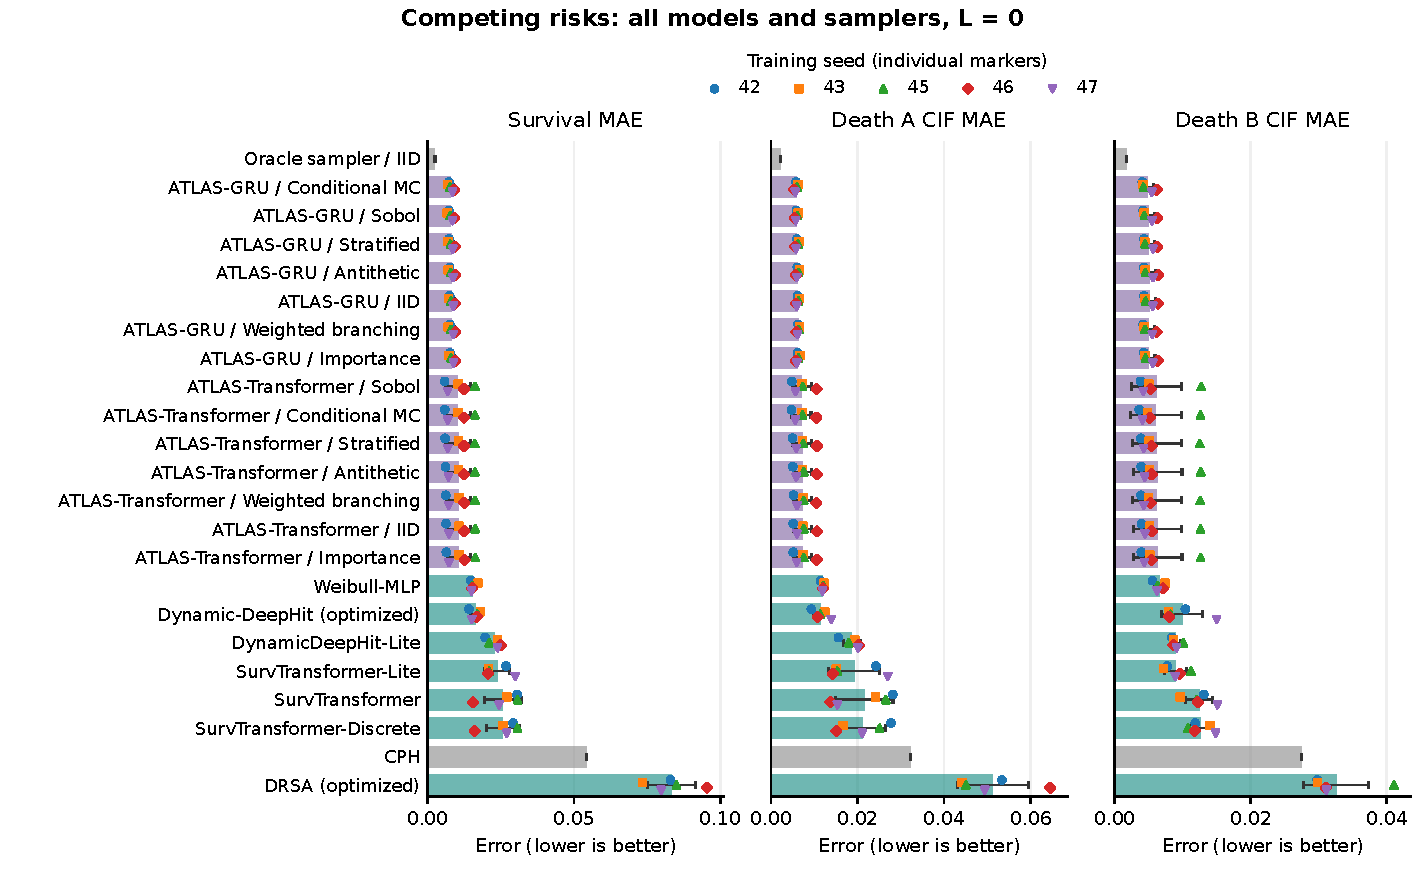
\includegraphics[width=0.95\linewidth,height=0.80\textheight,keepaspectratio]{cr3_five_seed_comparison_L0.pdf}\par
\captionof{figure}{Five-training-run comparison at $L=0$ in the multi-covariate competing-risks experiment. The panels show survival, Death A cumulative incidence and Death B cumulative incidence MAE. Bars are means across training runs; markers show individual runs and error bars show one sample standard deviation across runs. Each stochastic training-run score averages five sampling seeds at $M=10{,}000$. These are training-run standard deviations, not confidence intervals or within-run sampling standard deviations. CPH predictions agree to numerical precision; the oracle is a reused sampling control. Dynamic-DeepHit (optimized) and DRSA (optimized) use the validation-selected fits, and row order follows the updated mean survival MAE. Lower error is better.}\label{fig:cr3_five_L0}\par
\clearpage
\noindent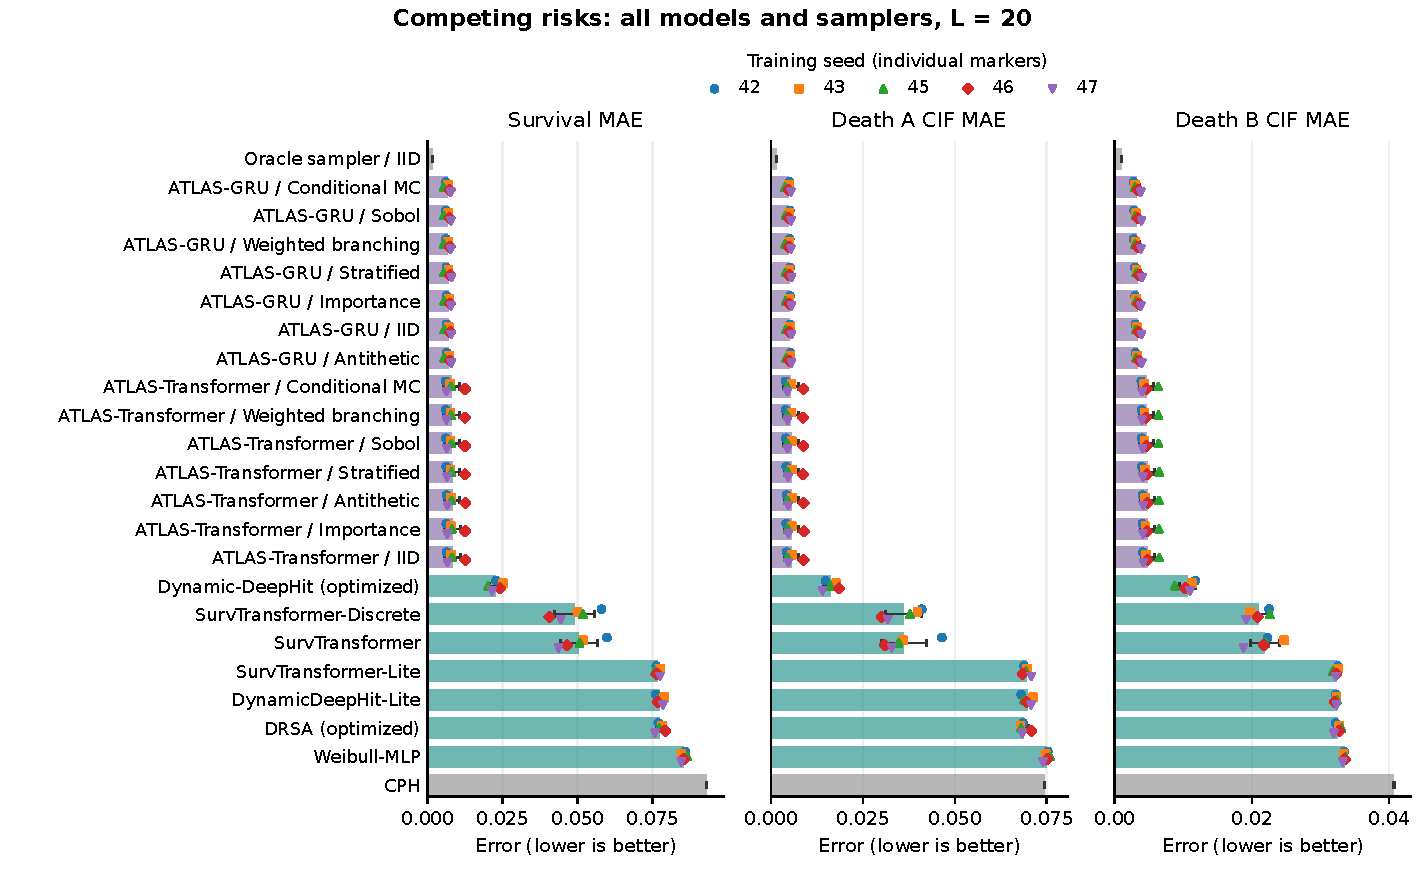
\includegraphics[width=0.95\linewidth,height=0.80\textheight,keepaspectratio]{cr3_five_seed_comparison_L20.pdf}\par
\captionof{figure}{Five-training-run comparison at $L=20$ in the multi-covariate competing-risks experiment. The panels show survival, Death A cumulative incidence and Death B cumulative incidence MAE. Bars are means across training runs; markers show individual runs and error bars show one sample standard deviation across runs. Each stochastic training-run score averages five sampling seeds at $M=10{,}000$. These are training-run standard deviations, not confidence intervals or within-run sampling standard deviations. CPH predictions agree to numerical precision; the oracle is a reused sampling control. Dynamic-DeepHit (optimized) and DRSA (optimized) use the validation-selected fits, and row order follows the updated mean survival MAE. Lower error is better.}\label{fig:cr3_five_L20}\par
\clearpage
\restoregeometry
\paperwidth=8.5in\paperheight=11in
\ifdefined\pdfpagewidth\pdfpagewidth=\paperwidth\pdfpageheight=\paperheight
\else\ifdefined\pagewidth\pagewidth=\paperwidth\pageheight=\paperheight
\else\special{papersize=8.5in,11in}\fi\fi
\endgroup
